\subsection{Questionnaire}

\textbf{Selection Rationale:} Questionnaires were used to obtain statistical evidence (n=25) for key assumptions identified during interviews, using primarily closed questions (multiple choice, Likert scales) to quantify findings such as single store shopping preference, time burden, and interest in CookWise.

\vspace{0.4cm}

\textbf{Execution:}

\begin{itemize}
    \item \textbf{Method:} Face-to-face questionnaire administered over a two week period
    \item \textbf{Locations:} BTH University campus and local gym in Karlskrona
    \item \textbf{Participants:} 25 individuals (12 university students, 3 professionals, 10 household members)
    \item \textbf{Questionnaire Design:} 15 questions (see Appendix A) organized into five sections: demographics, shopping behaviors, price sensitivity, meal planning habits, and interest in CookWise concept
    \item \textbf{Question Types:} Primarily closed questions (multiple choice, Likert scales 1-5) with limited open-ended questions
    \item \textbf{Duration:} 5-8 minutes per questionnaire
\end{itemize}

\textbf{Requirements Validated:}

The questionnaire provided quantitative validation for key requirements:

\begin{table}[h]
\centering
\caption{Requirements Validated Through Questionnaire}
\begin{tabular}{|l|p{9cm}|}
\hline
\textbf{Req ID} & \textbf{Validation Evidence} \\
\hline
\multicolumn{2}{|l|}{\textit{\textbf{Domain Requirements}}} \\
\hline
DL3 & Single store preference: 92\% always shop at one store, 8\% rarely visit multiple \\
\hline
\multicolumn{2}{|l|}{\textit{\textbf{Product Requirements}}} \\
\hline
PR2 & High interest in sale based recipe suggestions: 77\% rated 4 to 5 out of 5 \\
\hline
PR3 & Dietary filters important: 58\% indicated dietary restrictions or preferences \\
\hline
PR9 & Want to see savings details: 83\% said transparency in savings calculation is important \\
\hline
\multicolumn{2}{|l|}{\textit{\textbf{Quality Requirements}}} \\
\hline
QR1 & Time savings valued: 54\% spend 30+ minutes weekly on meal planning \\
\hline
QR2 & Usability important: Users want simple, intuitive interface \\
\hline
\end{tabular}
\end{table}

\vspace{0.2cm}

\textbf{Key Findings:}

\textbf{Finding 1: Time Burden Confirmed}

54\% of respondents spend 30+ minutes weekly on meal planning and grocery list preparation (mean: 37 minutes/week). This validates the system's focus on reducing planning time by 60 to 80\%.

\begin{figure}[H]
\centering
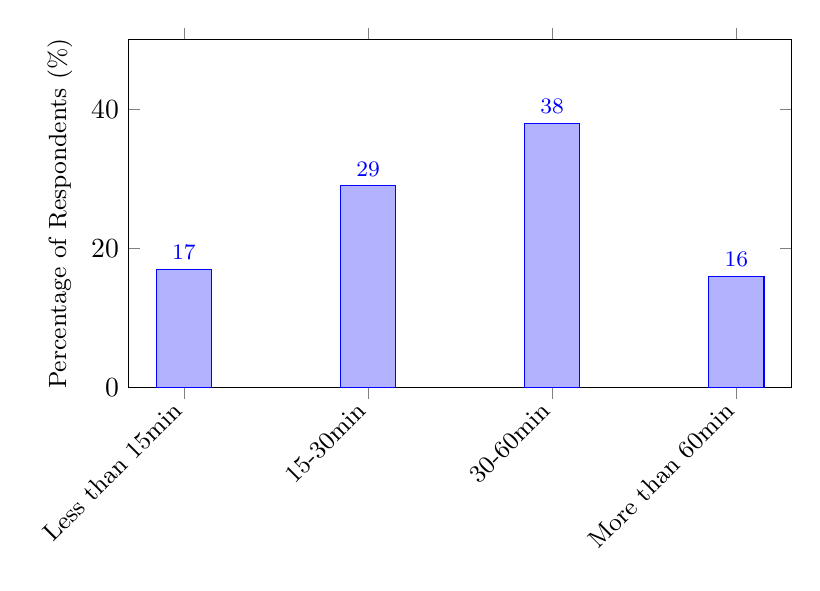
\begin{tikzpicture}
\begin{axis}[
    ybar,
    width=10cm,
    height=6cm,
    symbolic x coords={Less than 15min, 15-30min, 30-60min, More than 60min},
    xtick=data,
    x tick label style={font=\small, rotate=45, anchor=east},
    ylabel={Percentage of Respondents (\%)},
    ylabel style={font=\small},
    ymin=0, ymax=50,
    bar width=20pt,
    nodes near coords,
    every node near coord/.append style={font=\footnotesize},
]
\addplot coordinates {
    (Less than 15min,17) 
    (15-30min,29) 
    (30-60min,38) 
    (More than 60min,16)
};
\end{axis}
\end{tikzpicture}
\caption{Time Spent Weekly on Meal Planning and Grocery List Preparation}
\end{figure}

\textbf{Finding 2: Single Store Preference Validated}

92\% always shop at one store, 8\% rarely visit multiple stores (only in rare cases), and 0\% frequently shop at multiple stores. This strongly validates DL3 (single store constraint) as a fundamental requirement - virtually all users prefer single-store shopping, with no one regularly visiting multiple stores.

\begin{figure}[H]
\centering
\begin{tikzpicture}
\pie[
    text=legend,
    radius=2.5,
    color={green!60, yellow!60}
]
{92/Always one store, 8/Rarely multiple}
\end{tikzpicture}
\caption{Shopping Behavior: Single Store vs Multiple Stores}
\end{figure}

\textbf{Finding 3: High Interest in Sale Based Recipes}

When asked about interest in an app that automatically suggests recipes based on current sales, 77\% expressed high interest (rating 4 to 5 on a 5 point scale), with mean interest of 4.2/5.0. This validates PR2 (AI recipe suggestions based on sales) as a compelling core value proposition.

\begin{figure}[H]
\centering
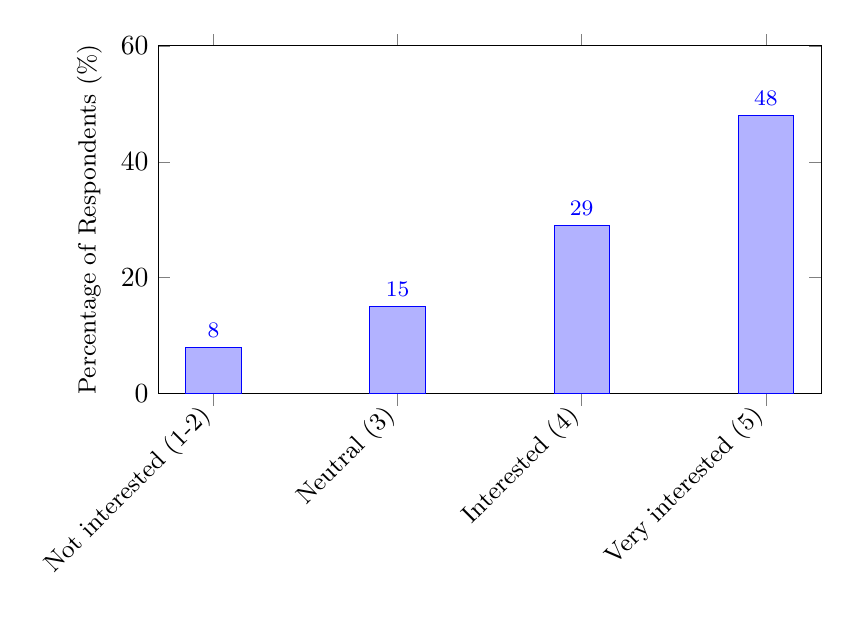
\begin{tikzpicture}
\begin{axis}[
    ybar,
    width=10cm,
    height=6cm,
    symbolic x coords={Not interested (1-2), Neutral (3), Interested (4), Very interested (5)},
    xtick=data,
    x tick label style={font=\small, rotate=45, anchor=east},
    ylabel={Percentage of Respondents (\%)},
    ylabel style={font=\small},
    ymin=0, ymax=60,
    bar width=20pt,
    nodes near coords,
    every node near coord/.append style={font=\footnotesize},
]
\addplot coordinates {
    (Not interested (1-2),8) 
    (Neutral (3),15) 
    (Interested (4),29) 
    (Very interested (5),48)
};
\end{axis}
\end{tikzpicture}
\caption{Interest Level in Sale Based Recipe Suggestions}
\end{figure}


\textbf{Key Insights:}

The questionnaire (n=25) quantitatively validated interview findings:

\begin{enumerate}
    \item Time burden confirmed: 54\% spend 30+ minutes weekly on meal planning.

    \item Single store preference validated: 92\% always shop at one store, confirming DL3 as fundamental constraint.

    \item High interest in CookWise: 77\% rated interest as 4 to 5 out of 5, demonstrating strong product market fit.
\end{enumerate}

\vspace{0.5cm}

\textbf{Limitations:} Limited sample size (n=25), convenience sampling at university/gym locations, self-report bias, and geographic limitation to Karlskrona area.

The complete questionnaire with all 15 questions is provided in Appendix A.